\documentclass[report.tex]{subfiles}
\begin{document}
\subsection{Methodology}
The RF filters discussed in this report can be divided in 3 sections
\begin{itemize}
    \item Lumped 2\nd order maximally flat band-pass filter
    \item Distributed 2\nd order maximally flat band-pass filter on RO4350B or FR-4 substrate
    \item Distributed maximally flat band-pass filter on FR-4 substrate (DesignGuide optimized filter order)
\end{itemize}
For each filter design, the attenuation at the pass- and stop-band limits (table \ref{table:filter specs}) was measured. A summary of measured attenuation is found in table \ref{table:attenuation summary}.

All filters were designed using ADS DesignGuide (\emph{Filter/Filter Control Window} or \emph{Passive Circuit/Microstrip Control Window}).

Two different types of simulations was performed on the distributed filters: schematic and layout simulation. The Schematic simulation can be launched directly from the DesignGuide control window. To do a layout simulation, a layout has to be either created or generated.

The layouts in this report were generated by first designing the filter with DesignGuide, \emph{push into hierarchy} of the filter and then select \emph{Layout/(Generate/Update layout)}. The substrate of the layout was then imported from the main schematic.

The layout simulation can then be launched from the menu of the layout design window. All layout simulations in this report are performed on a [1.0,3.0] GHz frequency span.

\subsubsection{Lumped 2\nd order maximally flat band-pass filter}
From the DesignGuide \emph{Filter/Filter Control Window}, a double terminated bandpass filter was chosen (see fig.~\ref{fig:Filter A}) and the specifications from table~\ref{table:filter specs} was filled in. The filter order was also entered. The simulation frequency span was automatically determined by DesignGuide to [1.94,2.94] GHz.

\begin{figure}[H]
    \centering
    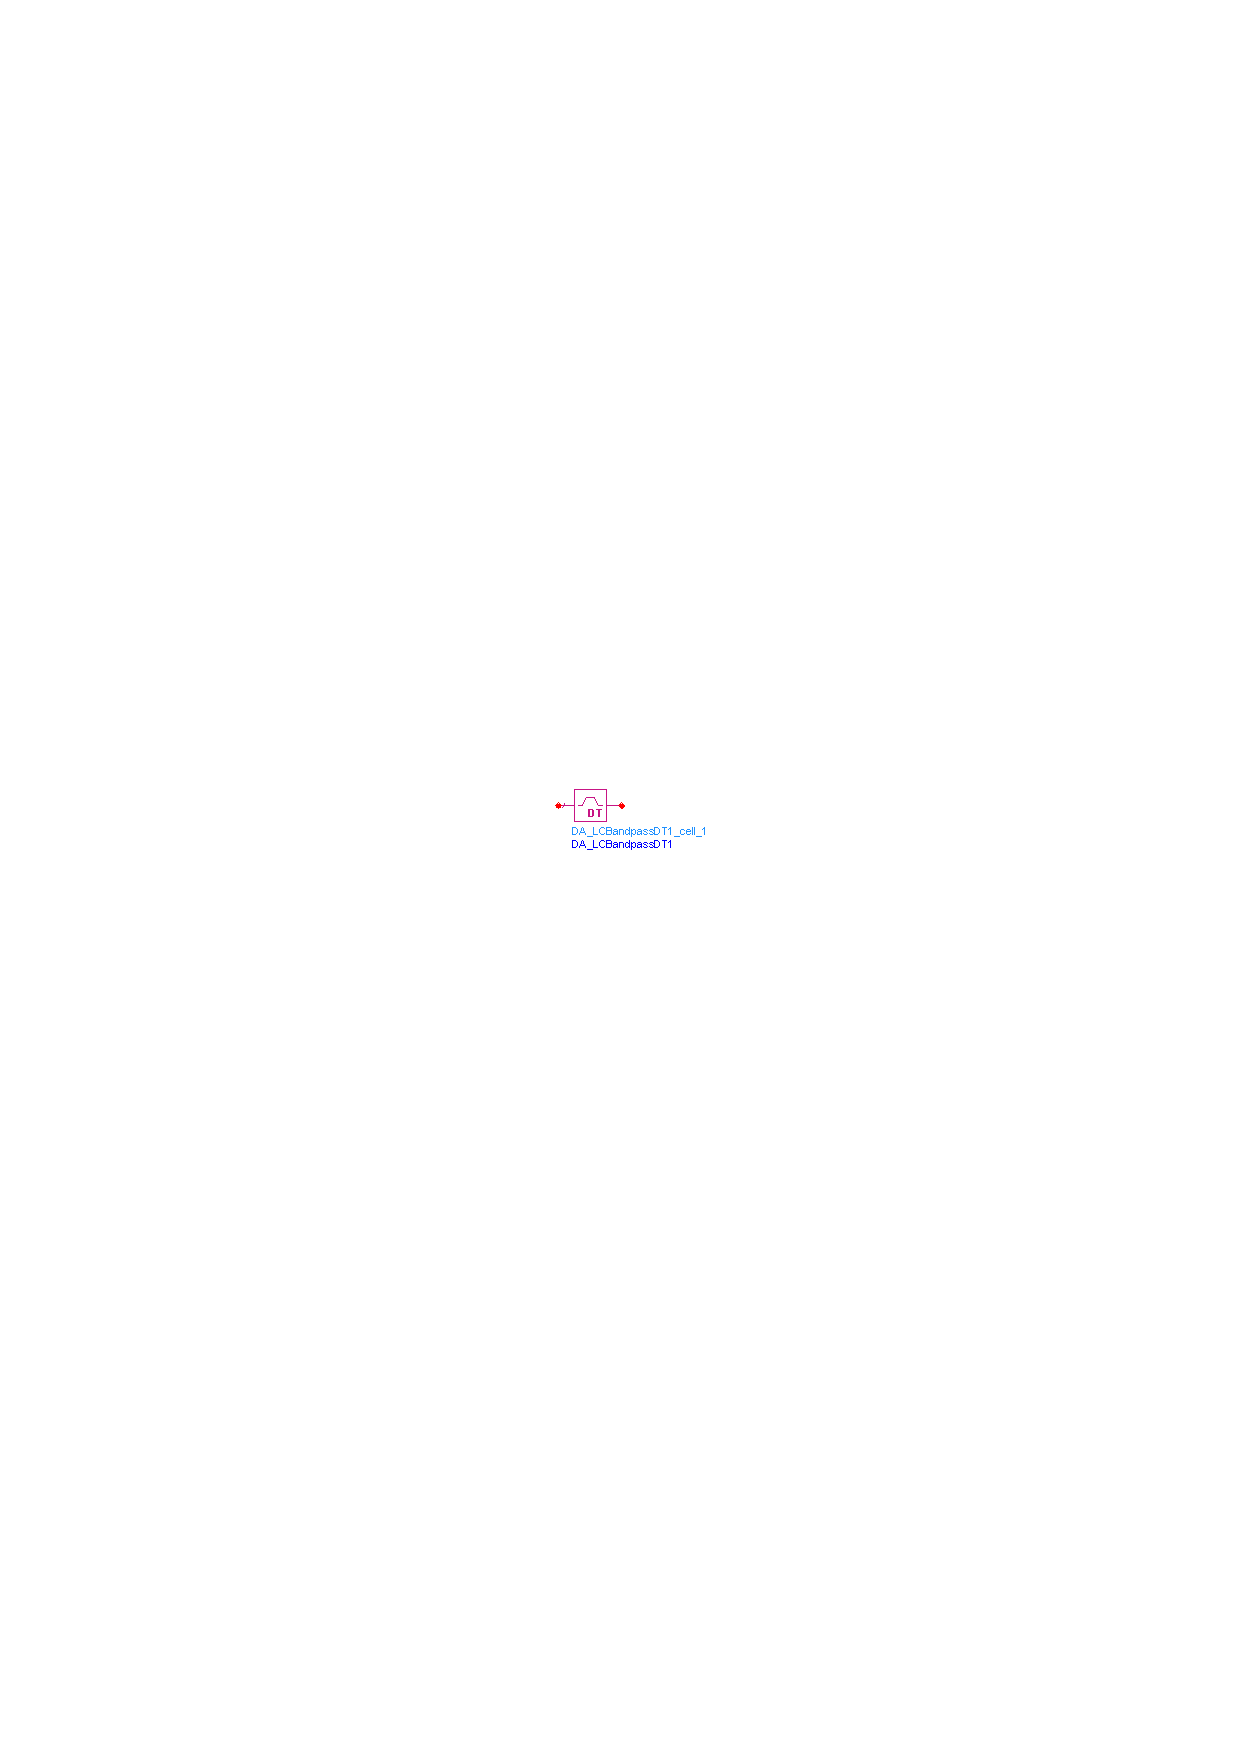
\includegraphics[scale=2]{design_guide_symbol}
    \caption{Double terminated bandpass filter schematic symbol}
    \label{fig:Filter A}
\end{figure}

\subsubsection{Distributed 2\nd order maximally flat band-pass filter on RO4350B or FR-4 substrate}
From the DesignGuide \emph{Passive Circuit/Microstrip Control Window}, Microstrip Coupled-line filter was chosen (see fig.~\ref{fig:Filter B schematic} and \ref{fig:Filter C schematic}), the specifications from table~\ref{table:filter specs} was filled in, and the appropriate substrates were added with the specifications from table~\ref{table:substrate specs}. The filter order was also entered.

\begin{figure}[h]
    \centering
    \subfloat[]{
        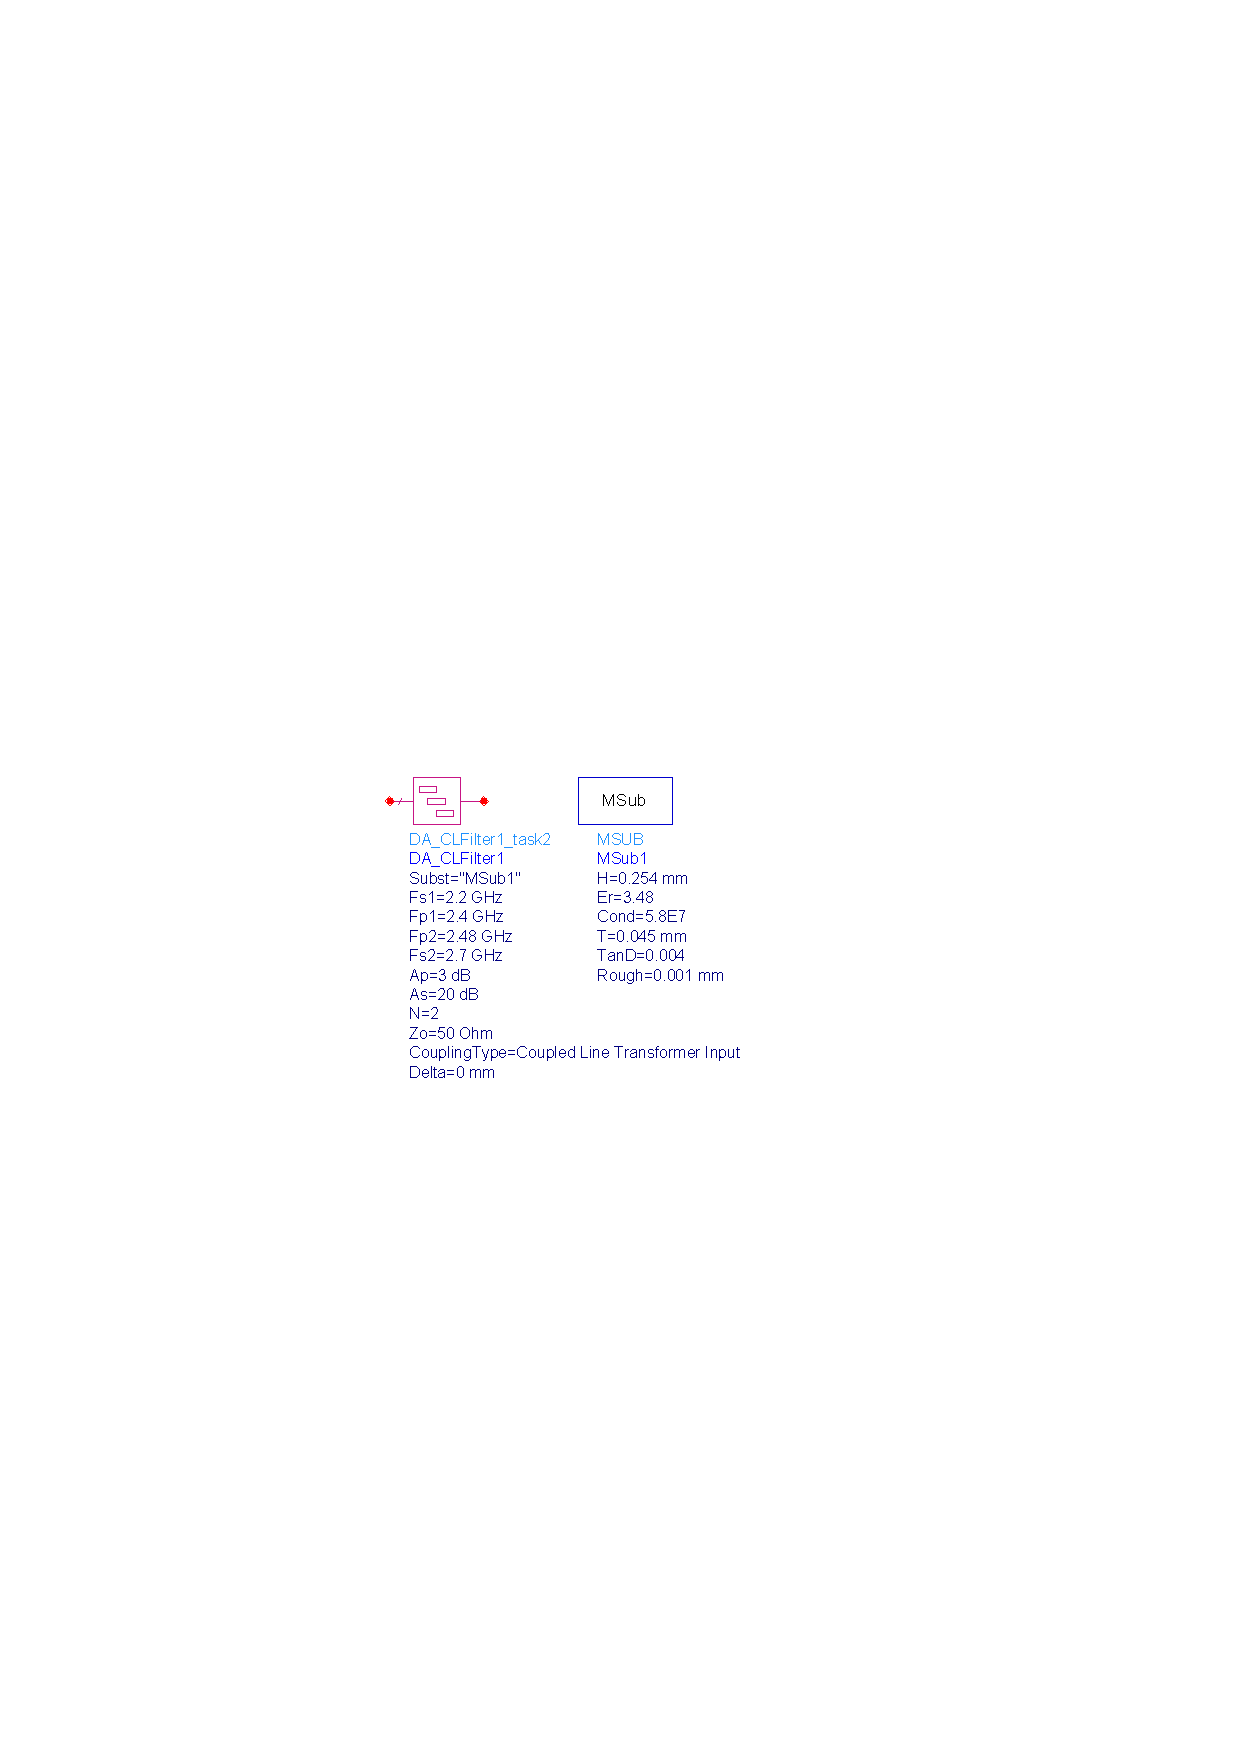
\includegraphics[width=0.4\linewidth]{filter_B_schematic}
    }
    \subfloat[]{
        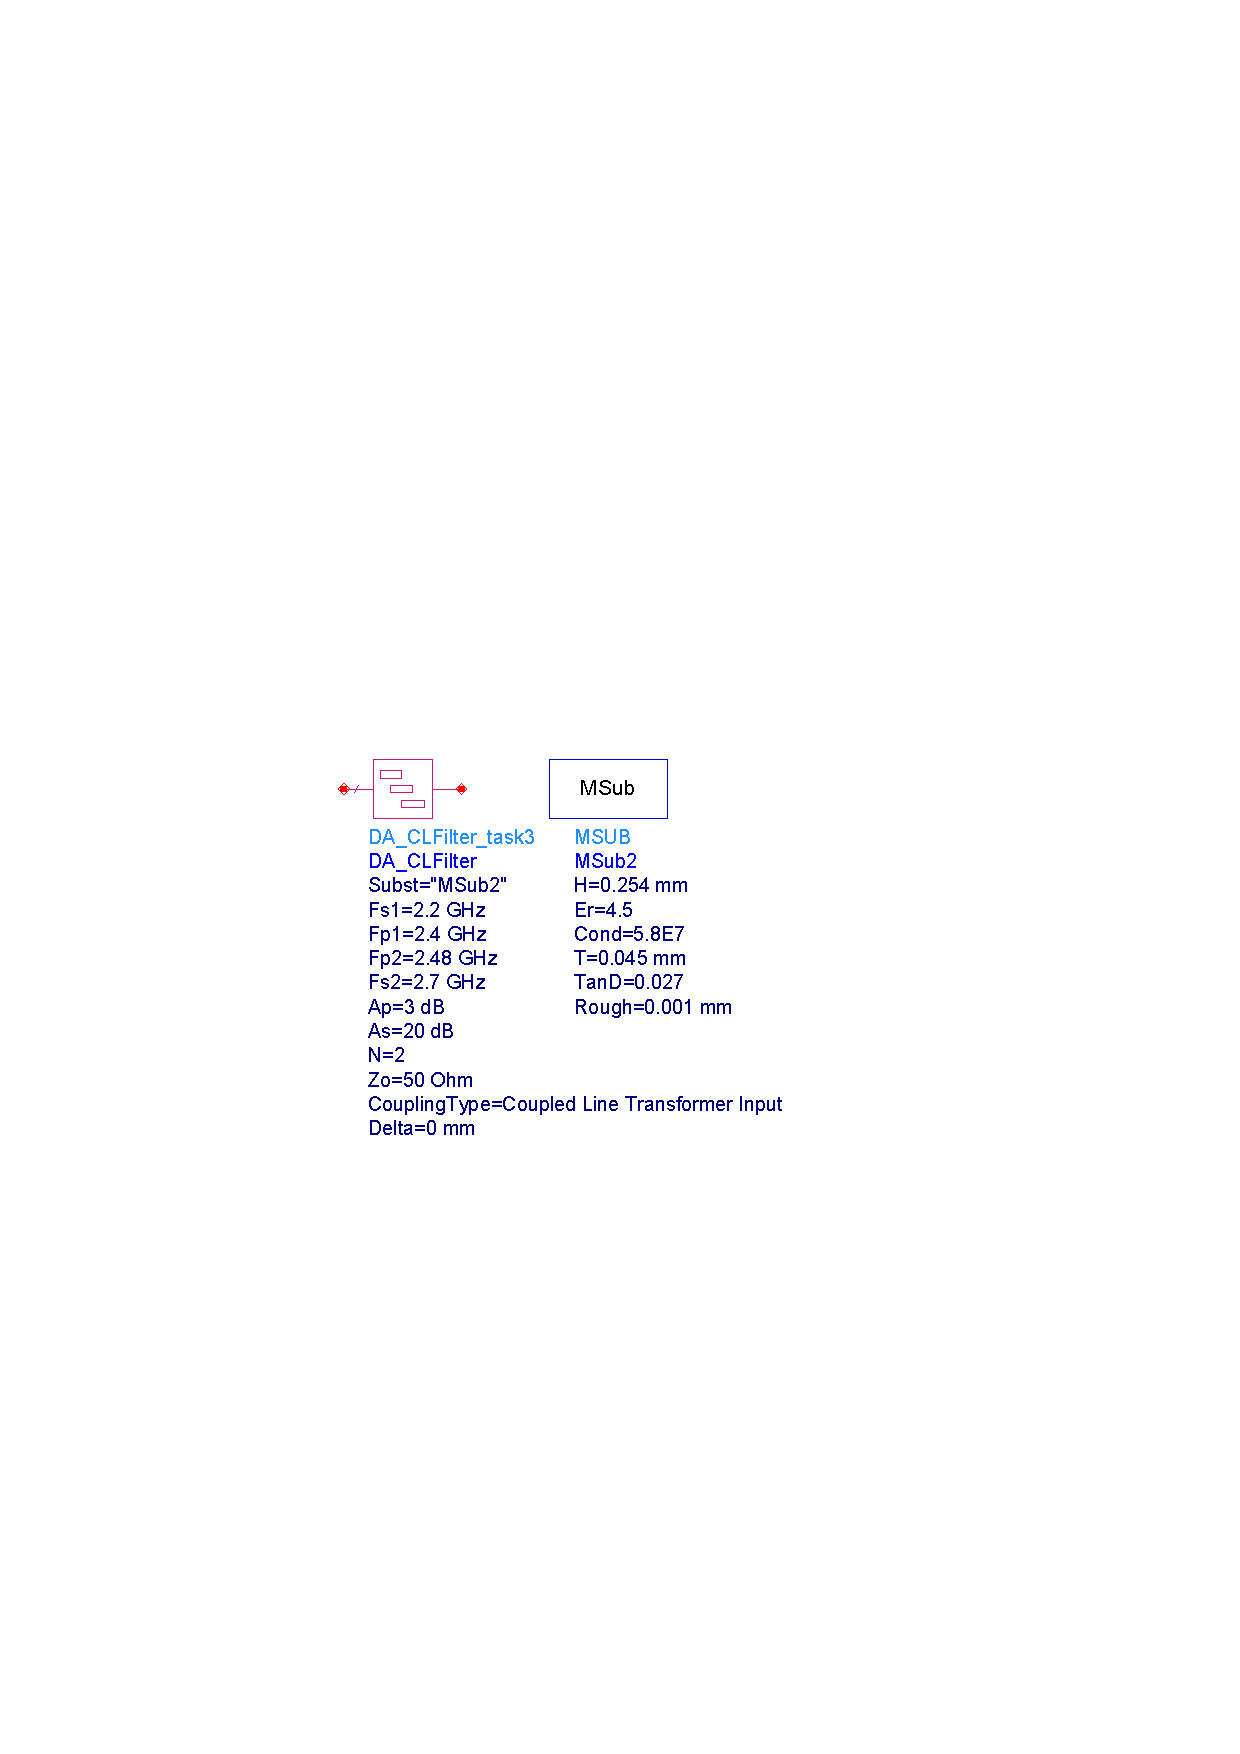
\includegraphics[width=0.4\linewidth]{filter_C_schematic}
    }
    \caption{Microstrip Coupled-line filter with (a) RO4350B and (b) FR-4}
    \label{fig:Filter B schematic}
\end{figure}

Pushing into hierarchy give the layout schematic shown in fig.~\ref{fig:Filter B layout schematic} (RO4350B), which will generate the microstrip layout shown in fig.~\ref{fig:Filter B layout}.

\begin{figure}[h]
    \centering
    \subfloat[Layout schematic] {
        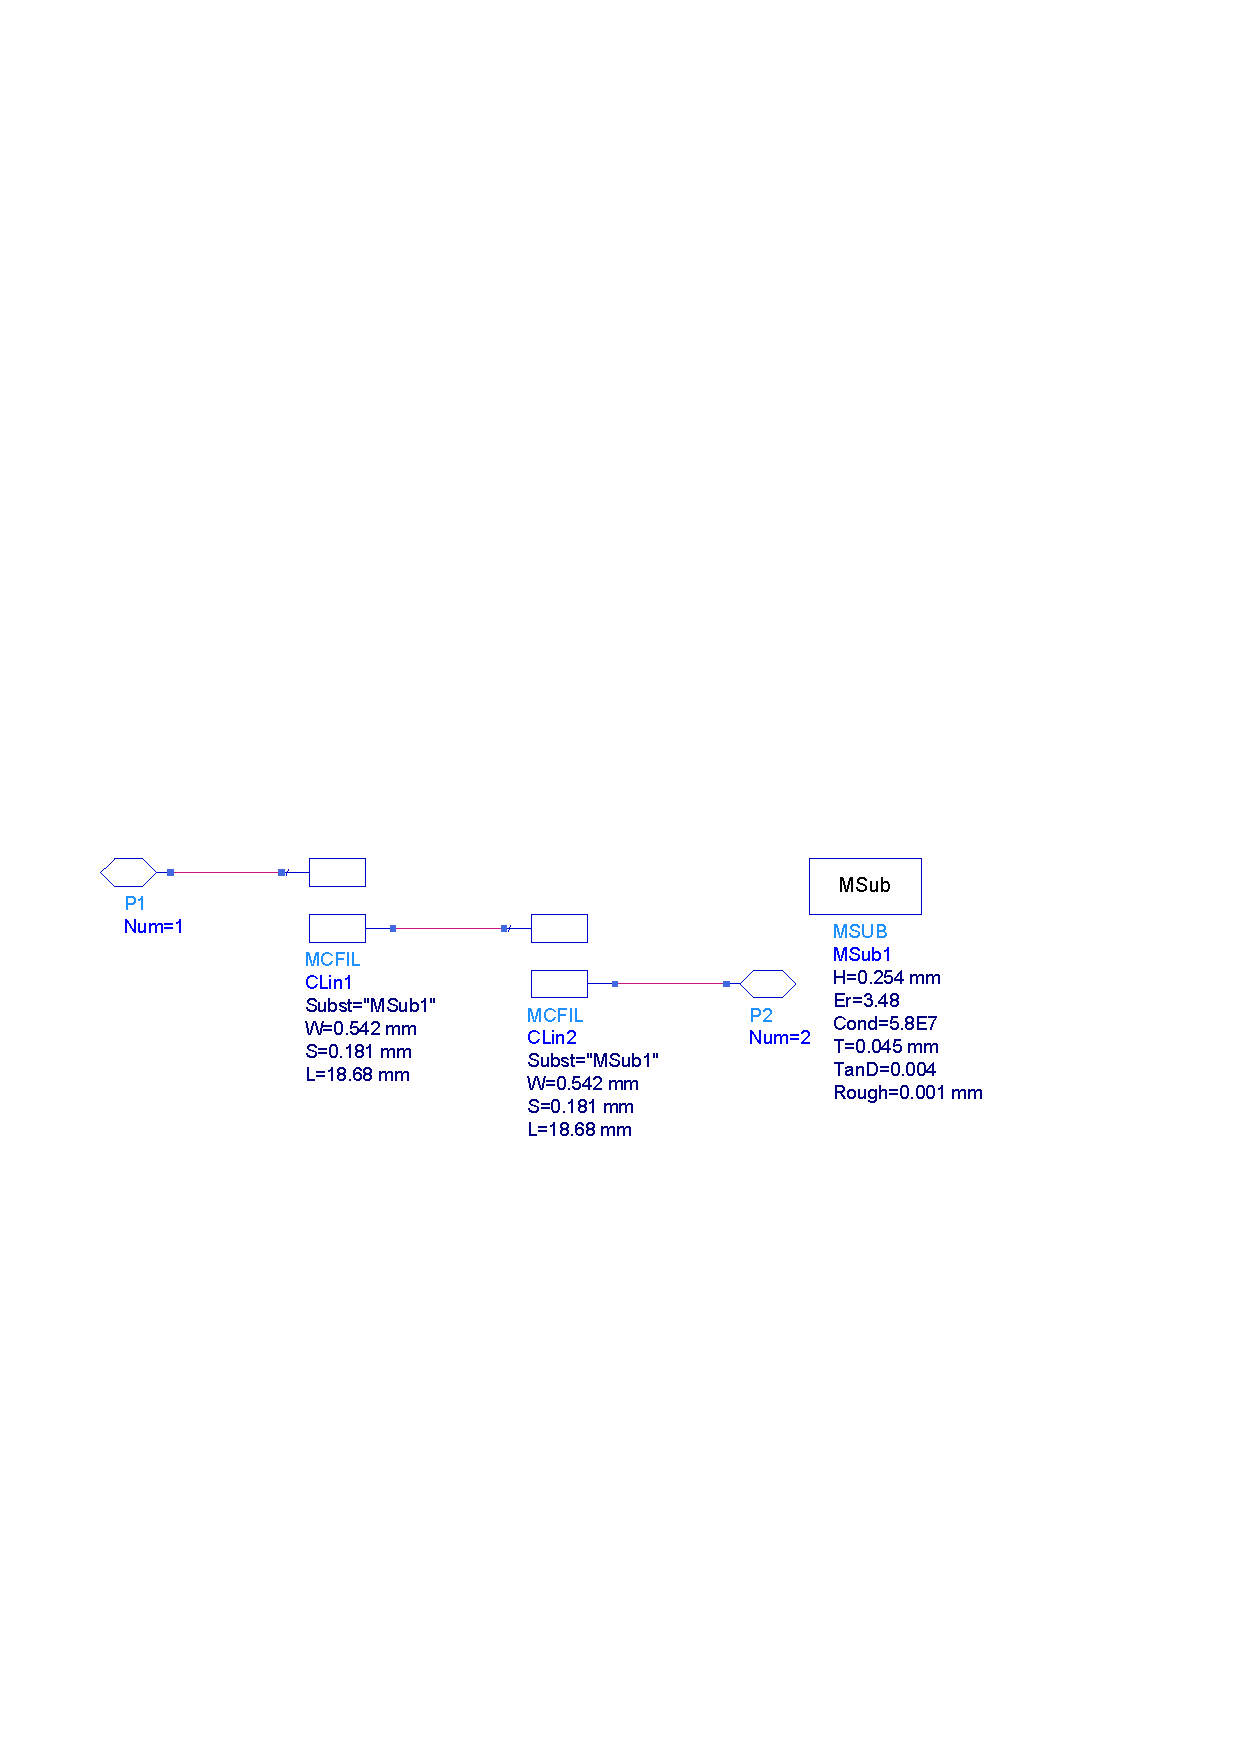
\includegraphics[width=0.8\linewidth]{filter_B_layout_schematic}
        \label{fig:Filter B layout schematic}
    }
    
    \subfloat[Microstrip layout]{
        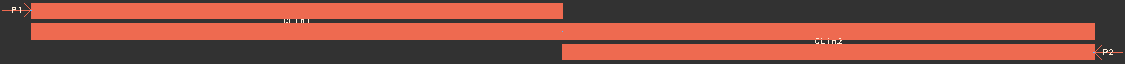
\includegraphics[width=0.8\linewidth]{filter_B_layout}
        \label{fig:Filter B layout}
    }
    \caption{Schematic and layout of microstrip Coupled-line filter (RO4350B)}
\end{figure}

The schematic and layout in fig.~\ref{fig:Filter B layout schematic} and fig.~\ref{fig:Filter B layout} will be identical for FR-4

\subsubsection{Distributed 2\nd order maximally flat band-pass filter (FR-4)}
By changing the filter order in fig~\ref{fig:Filter B schematic} from N=2 to N=0, DesignGuide will automatically try to determine the lowest order needed to meet the filter specifications. The resulting layout schematic and microstrip layout can be seen in fig.~\ref{fig:Filter C layout schematic auto-N} and \ref{fig:Filter C layout auto-N}.

\begin{figure}[h]
    \centering
    \subfloat[Layout schematic] {
        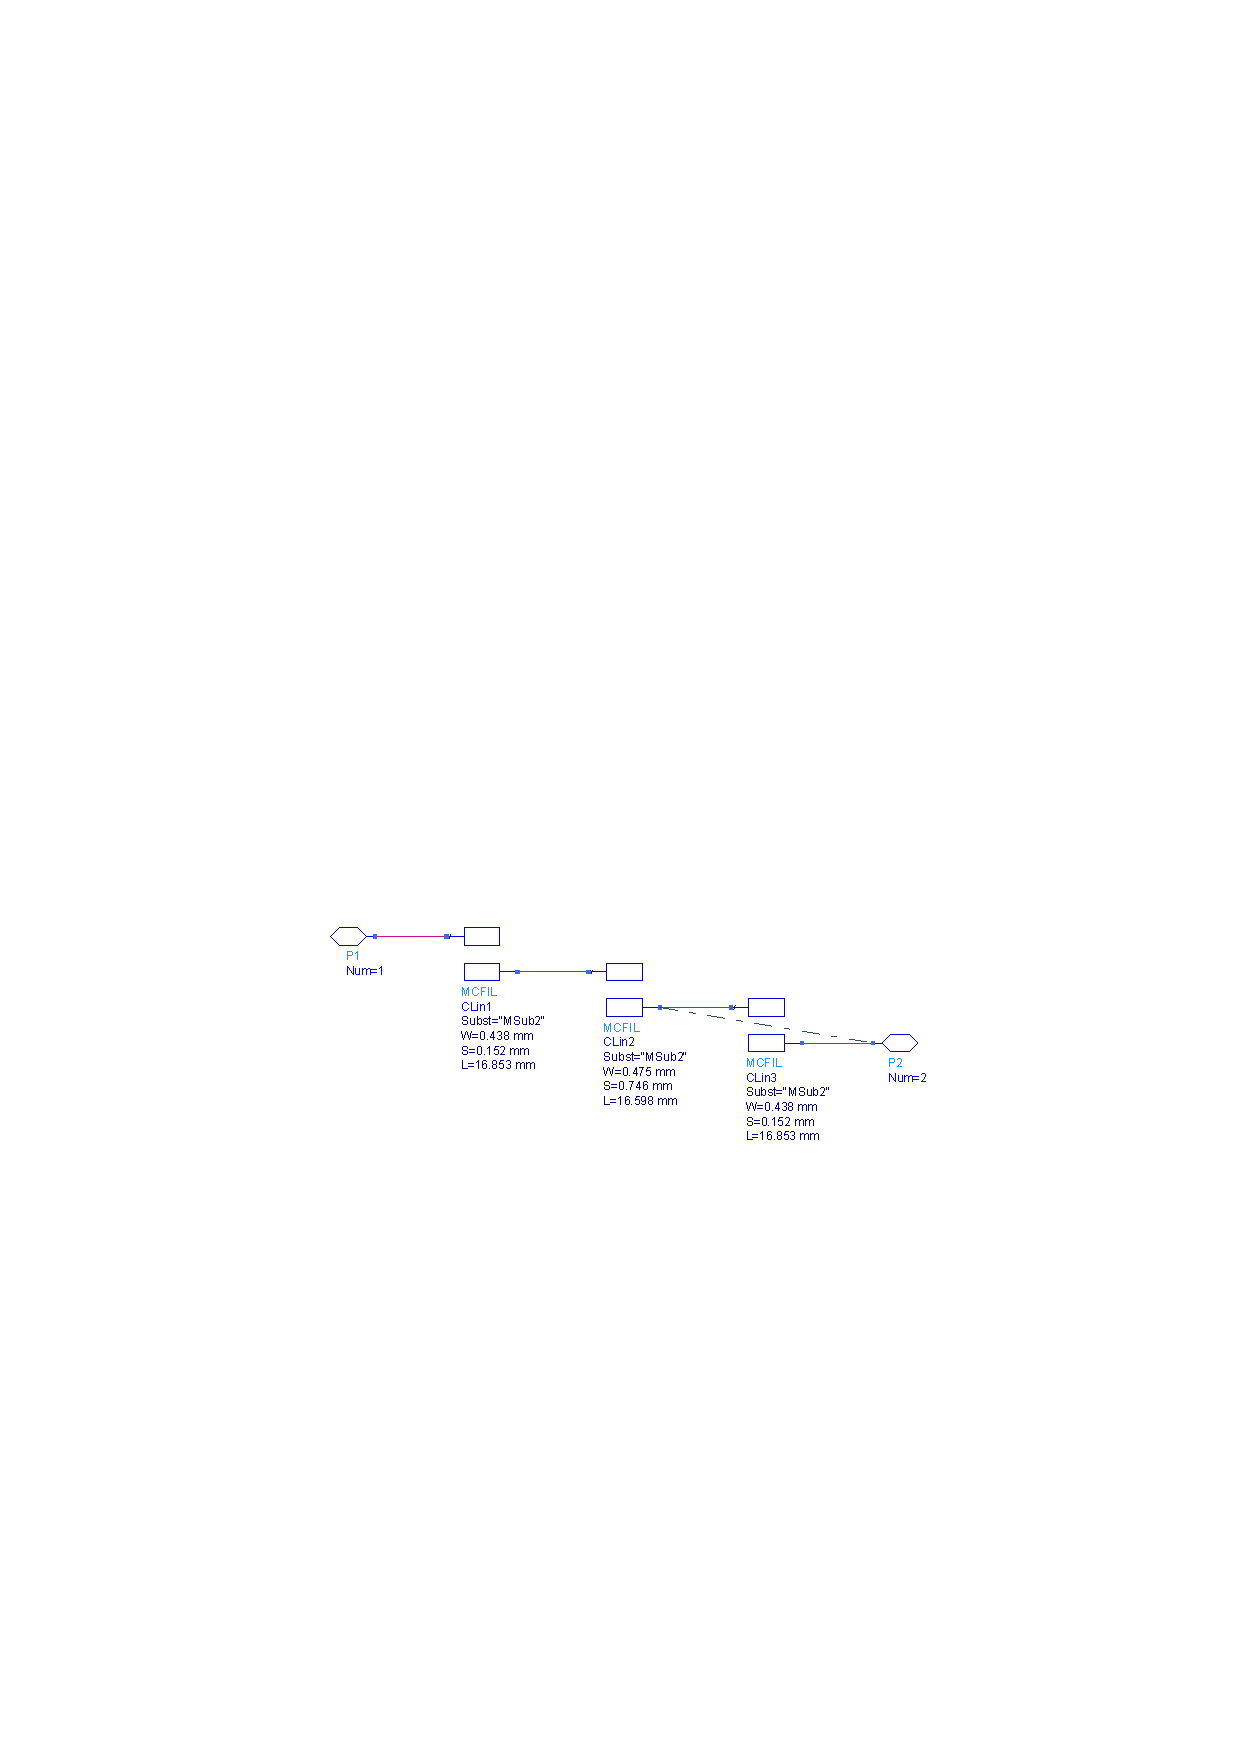
\includegraphics[width=0.8\linewidth]{filter_C_layout_schematic_auto-N}
        \label{fig:Filter C layout schematic auto-N}
    }
    
    \subfloat[Microstrip layout]{
        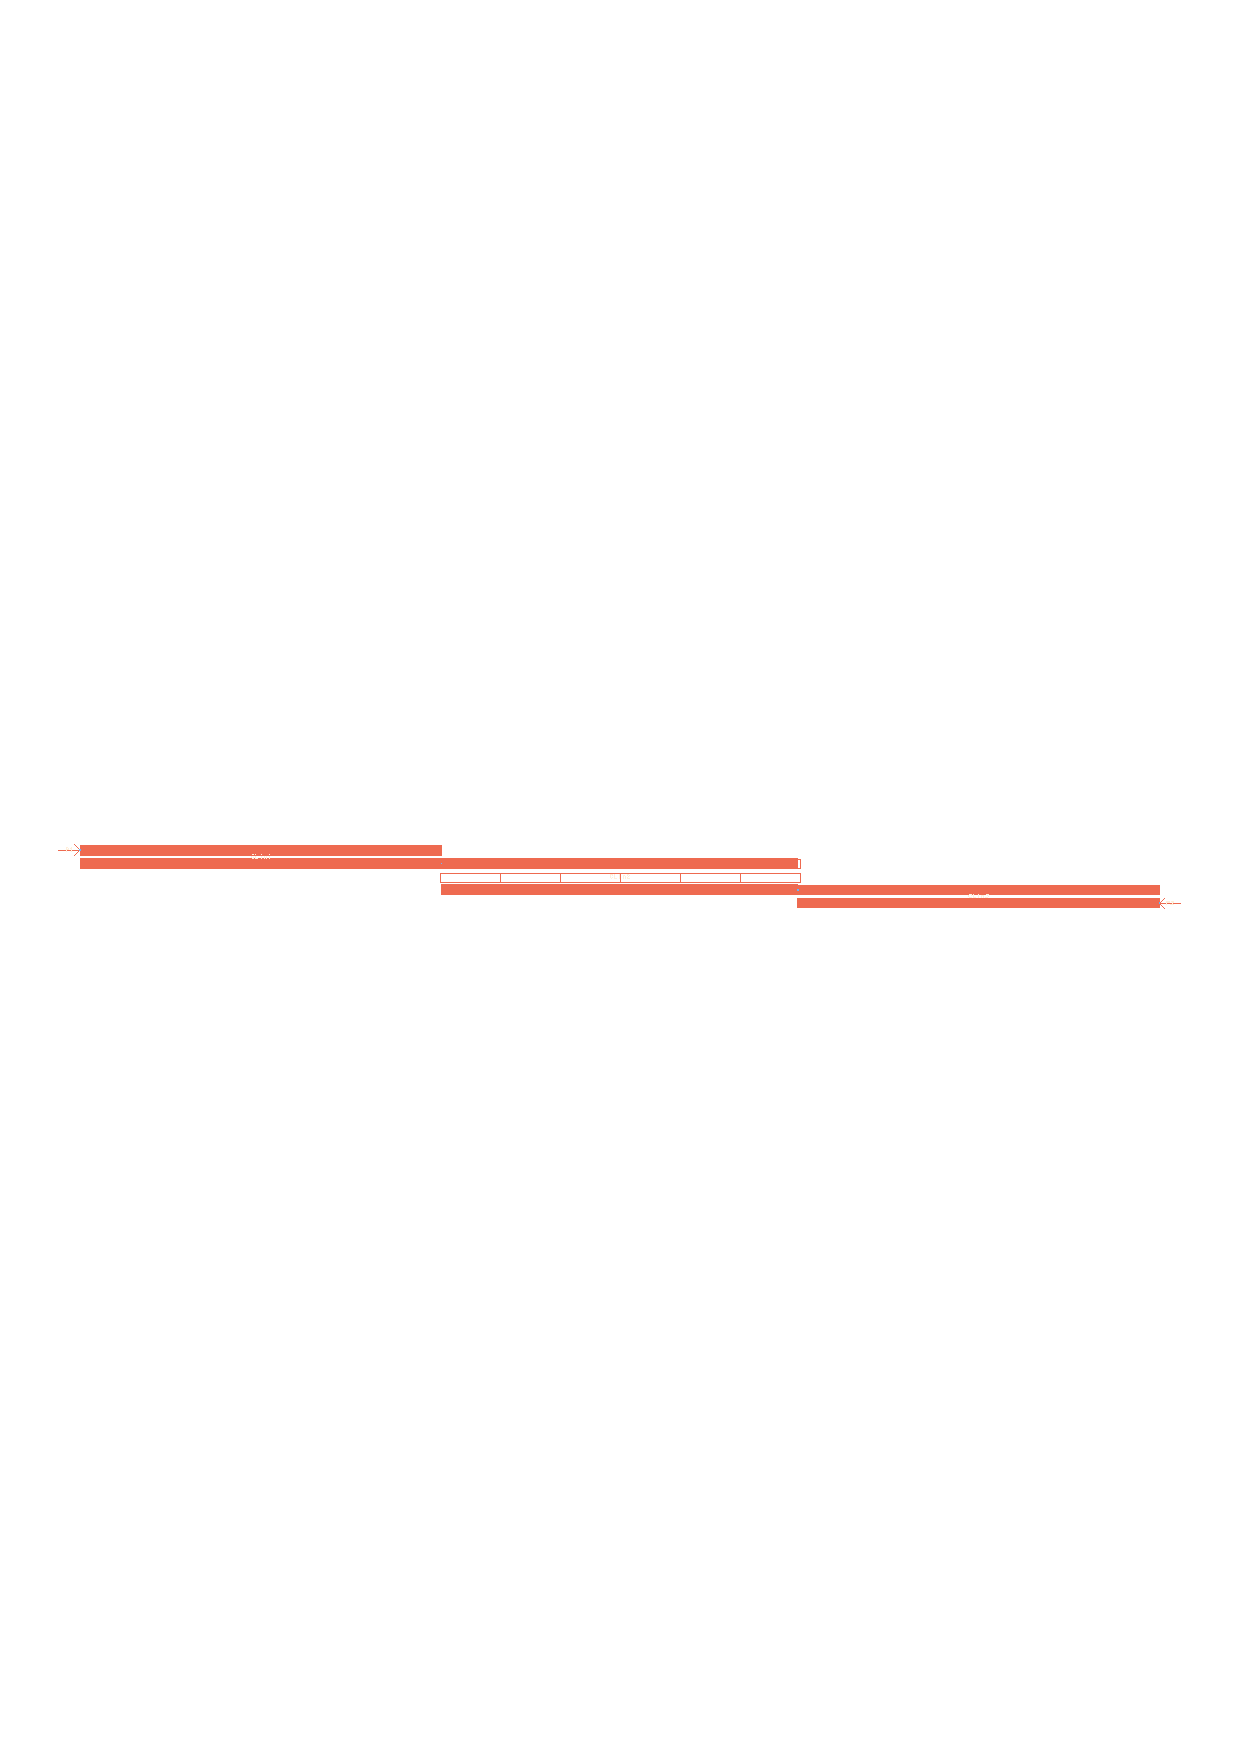
\includegraphics[width=0.8\linewidth]{filter_C_layout_auto-N}
        \label{fig:Filter C layout auto-N}
    }
    \caption{Schematic and layout of microstrip Coupled-line filter (RO4350B)}
\end{figure}

\end{document}